\chapter{WORK PACKAGE 3}
    In questo capitolo si andrà a sottoporre ad analisi la soluzione proposta nel WP2 tenendo conto delle proprietà espresse all’interno del WP1, ovvero \textit{confidenzialità}, \textit{integrità}, \textit{trasparenza} ed \textit{efficienza}.

    \section{Confidenzialità}
        \begin{itemize}
            \item \textbf{Malevolent Server} \\
                Questa tipologia di attaccante mina la confidenzialità delle informazioni trasferite dall'utente al server erogatore del servizio, essendo quest'ultimo capace di visionare in chiaro le credenziali interne al certificato.
                Il server malevolo potrebbe, quindi, collezionare i dati al fine di utilizzarli per scopi illeciti.

            \item \textbf{Identity Thief} \\
                Questo avversario, una volta ottenute le informazioni circa l'identità o la credenziale relativa ad un utente, può richiedere in maniera fraudolenta l'accesso ad un determinato servizio.
                Le informazioni sugli utenti possono essere ottenute per via traverse, come data leak o data breach, o tramite attacco man-in-the-middle.
                L'adozione di canali TLS di comunicazione, impedisce tale tipo di attacco; inoltre, pur avendo possesso di informazioni personali, non è possibile dimostrare l'identità se non si possiede anche la chiave privata, in quanto l'algoritmo di verifica della firma di Schnorr richiede tale passaggio.

            \item \textbf{The Eavesdropper \& Data Miner} \\
                Questo tipo di malintenzionati possono mettersi in ascolto sul canale di comunicazione cercando di carpire informazioni personali con l'intento di raccoglierle o rivenderle.
                Anche questi tipi di attacco non hanno successo, in quanto, come detto in precedenza, i canali di comunicazione sono tutti canali sicuri TLS.

            \item \textbf{Evil Insider} \\
                L'attaccante in questione può condurre attacchi sia verso utenti sia verso autorità o server, poiché è un operatore interno.
                Nello specifico, per quanto concerne i danni arrecati agli utenti, l'\textit{Evil Insider} può effettuare un'esfiltrazione dei dati personali o delle credenziali per fini illegittimi.

            \item \textbf{The Data Harvesters} \\
                Questi attaccanti raccolgono grandi quantità di dati per analisi o rivendita.
                Nonostante la raccolta di dati in sé non sia sempre malevola, può portare a violazioni della privacy se i dati sono utilizzati senza il consenso dell'utente.
        \end{itemize}
        
        \noindent Analizzando le proprietà descritte nel WP1, è possibile notare che:
        
        \begin{enumerate}
            \item \textbf{C1:} questa proprietà viene garantita in quanto, grazie alla struttura di gestione delle informazioni personali, l’utente fornisce tramite certificato i propri dati anagrafici solo alle CA fidate, mentre ai server invia i certificati contenenti solo la credenziale necessaria per l'accesso al servizio specifico

            \item \textbf{C2 - C3:} le proprietà in esame vengono garantite grazie alla presenza di un canale di comunicazione basato su TLS sia tra l’utente e le CA sia tra l’utente e i server

            \item \textbf{C4:} tale proprietà è garantita \textbf{a patto che l’utente non ceda volontariamente o venda le proprie chiavi private}, associate alle chiavi pubbliche presenti nella CIE e/o sulle credenziali.
            Tuttavia, in codesti casi, le precauzioni adottate possono intervenire in favore, in quanto:
            \begin{itemize}
                \item \textit{se l’utente non cede volontariamente} le proprie chiavi private, può richiedere una revoca dei certificati di cui ha notato un abuso, di modo da associare a questi ultimi delle nuove chiavi segrete;

                \item \textit{se l’utente cede volontariamente} queste informazioni non è possibile in alcun modo intervenire
            \end{itemize}
        \end{enumerate}

    \section{Integrità}
        \begin{itemize}
            \item \textbf{Evil Insider} \\
                Un insider malevolo mira ad alterare i dati critici sui server, come le credenziali degli utenti o i registri delle transazioni, compromettendo l'integrità del sistema.
                L'insider ha un accesso privilegiato e può modificare i dati senza essere immediatamente rilevato.

            \item \textbf{Identity Thief} \\
                Un ladro di identità può utilizzare credenziali rubate per accedere ai servizi e alterare i dati dell'utente legittimo o per falsificare la propria identità mascherandola con quella della vittima.
                Ad esempio, un attaccante di questo tipo potrebbe accedere al conto bancario di un utente e trasferire fondi senza autorizzazione.

            \item \textbf{The Cryptographer} \\
                Utilizzando attacchi crittografici avanzati, questo attaccante potrebbe alterare dati durante la trasmissione, compromettendo l'integrità delle informazioni.
                Potrebbe, ad esempio, utilizzare attacchi di tipo "man-in-the-middle" per alterare i messaggi scambiati tra due parti.

            \item \textbf{Crypto Conspirators} \\
                Questo gruppo di attaccanti potrebbe collaborare per compromettere i protocolli crittografici, permettendo la modifica dei dati durante la trasmissione. 
                Ad esempio, potrebbero introdurre una vulnerabilità in un protocollo di crittografia utilizzato per la comunicazione sicura tra utenti e server.
                Un caso d'esempio potrebbe essere rappresentato dalla possibilità che un gruppo di hacker riesca ad inserire una backdoor nel software crittografico utilizzato da una compagnia, ottenendo la capacità di alterare documenti riservati senza essere scoperti.
        \end{itemize}

        \noindent Analizzando le proprietà relative all'integrità, si ha:
        
        \begin{enumerate}
            \item \textbf{I1:} per quanto riguarda questo aspetto, si possono identificare due scenari:
                \begin{enumerate}
                    \item nel primo caso, si assumono come onesti tutti i componenti del sistema (utenti, CA, server).
                    In questo caso, non vi è alcun pericolo per l'integrità delle informazioni circolanti nei canali di comunicazione;

                    \item nel secondo caso, invece, assumendo un possibile attaccante all'interno dei server, non è possibile garantire l'integrità.
                    Si immagini un caso d'esempio tale per cui un attaccante interno (\textit{Evil Insider}) ad un server, visionando in chiaro le credenziali degli utenti, raccolga le informazioni sensibili al fine di strutturare il profilo dell'utente e rivendere i dati personali o utilizzarli per scopi illeciti. \\
                    A causa della centralizzazione del sistema non è possibile difendersi totalmente da questo tipo di attacchi, ma è possibile limitarli parzialmente tramite l'adozione di log, che vadano a mantenere una lista della transazioni effettuate, e controlli incrociati sulle attività svolte
                \end{enumerate}
            
            \item \textbf{I2:} l'adozione di diversi protocolli sicuri, come TLS per la trasmissione e lo schema di firma per i certificati, previene modifiche non autorizzate ai dati durante la trasmissione.
            Anche se un attaccante intercettasse i dati, non potrebbe alterarli senza che la modifica venga rilevata

            \item \textbf{I3:} tale proprietà è garantita dalla presenza, sulla CIE, di un certificato interno, firmato dall'IPZS, e un PIN associato alla scheda.
            Si è inoltre supposto che l'IPZS (che è una parte fidata) abbia rilasciato pubblicamente la procedura con cui la CIE viene costruita e firmata

            \item \textbf{I4:} questa proprietà viene garantita dalla firma, apposta da ogni utente sui certificati X.509v3, generata tramite lo schema di firma di Schnorr.
            Infatti, nel caso in cui il documento fosse stato rubato, sarebbe verificabile la sua validità ma non l'appartenenza al malintenzionato poiché, a fronte di una \textit{Zero Knowledge Proof}, non sarebbe in grado di provare ad un \textit{Verifier} che è a conoscenza dell’informazione segreta (la chiave privata $sk$) legata alla chiave pubblica, derivabile dalla firma, presente all’interno del documento
        \end{enumerate}

    \section{Trasparenza}
        \begin{itemize}
            \item \textbf{Anti-Tech Theorist} \\
                Diffondendo informazioni false o allarmistiche, può minare la fiducia degli utenti nella trasparenza del sistema.
                Si pensi ad un esempio in cui un oppositore all'avanzamento tecnologico vada a diffondere voci su vulnerabilità inesistenti in un sistema di autenticazione per generare panico e sfiducia tra gli utenti.

            \item \textbf{Evil Insider} \\
                Questo attaccante interno può manipolare i sistemi di autenticazione o di rilascio delle credenziali per nascondere le proprie attività malevole.
                Ad esempio, un dipendente con accesso privilegiato potrebbe modificare i log di accesso per nascondere il furto di dati sensibili, rendendo così difficile il rilevamento dell'attacco.

            \item \textbf{The Cryptographer} \\
                Utilizzando tecniche avanzate, questo attaccante potrebbe rendere difficile la verifica delle credenziali rilasciate, compromettendo la trasparenza del processo di autenticazione.
                Un attaccante, ad esempio, può falsificare dei certificati digitali, rendendo difficile per gli utenti e gli amministratori distinguere i certificati validi da quelli compromessi.

            \item \textbf{Identity Thief} \\
                Operando sotto identità rubate, questo attaccante rende complesso il tracciamento delle sue attività malevole, compromettendo la trasparenza generale del sistema.
        \end{itemize}

        \noindent Circa le proprietà inerenti alla trasparenza, è denotabile che:
        
        \begin{enumerate}
            \item \textbf{T1:} tale proprietà viene rispettata tramite l'utilizzo di librerie e tool open source, le quali permettono un'analisi accurata dei protocolli scelti, al fine di poter fornire prove di assenza di manomissione, dando motivo agli utenti di fidarsi del sistema

            \item \textbf{T2:} il rilascio di credenziali spetta solo alle CA, prese come parte fidata, limitando così la dipendenza da organi terzi e favorendo la velocità di verifica delle credenziali da parte dei server.
            Inoltre, l'adozione di log per le transizioni potrebbe migliorare ulteriormente questo scenario, sfavorendo la generazione di credenziali false o alterate

            \item \textbf{T3:} questa proprietà è garantita dall'architettura del sistema, in quanto ogni server, che eroga un servizio specifico, richiede delle credenziali all'utente, che desidera connettersi ad esso.
            Tuttavia, è possibile, da parte dell'utente, fornire solo ed esclusivamente le credenziali necessarie per l'accesso al servizio, evitando così di divulgare informazioni superflue alla fruizione

            \item \textbf{T4:} il sistema prevede l'utilizzo dello schema di firma di Schnorr in accoppiata con canali TLS, che garantisce l'autenticità della fonte tramite \textit{Zero Knowledge Proof}, per i certificati digitali.
            Inoltre, i certificati hanno una scadenza fissa e, come ulteriore protezione, nel caso in cui un utente notasse un abuso di credenziali legate al proprio profilo, potrebbe richiederne la revoca (e le CA hanno le CRL).
            
        \end{enumerate}

    \section{Efficienza}
        \begin{itemize}
            \item \textbf{The Denier} \\
                Un attaccante che nega l'autenticità dei certificati potrebbe sovraccaricare il sistema con richieste di verifica, riducendo l'efficienza.
                Un esempio potrebbe riguardare un possibile attacco di tipo denial-of-service (DoS), il quale potrebbe inondare i server di richieste di verifica delle credenziali.

            \item \textbf{Anti-Tech Theorist} \\
                Generando panico e disinformazione, questo attaccante può causare un aumento delle richieste di assistenza e verifiche, rallentando il sistema.
                La diffusione di notizie allarmistiche può portare a un sovraccarico dei canali di supporto.

            \item \textbf{Evil Insider} \\
                Introducendo backdoor o manipolando politiche di accesso, questo attaccante può causare rallentamenti o inefficienze nei processi di autenticazione e accesso ai servizi.
                Ad esempio, un dipendente malintenzionato potrebbe alterare le configurazioni del server di autenticazione, causando un aumento dei tempi di risposta e una riduzione della reattività del sistema.

            \item \textbf{The Cryptographer} \\
                L'ipotesi di un attacco ai canali TLS da parte di questo attaccante può introdurre sovraccarichi nei server e nella rete, causando un aumento del tempo di elaborazione per ogni richiesta e rallentando significativamente il sistema.
        \end{itemize}

        \noindent Analizzando le proprietà di efficienza descritte nel WP1, è possibile notare che:

        \begin{enumerate}
            \item \textbf{E1:} l'utilizzo di credenziali per l'accesso ai server, rende modulare la fruizione dei servizi, permettendo anche l'utilizzo di requisiti complessi (es. \verb|"Residente a Salerno" OR "Nato a Salerno"|).

            \item \textbf{E2:} la gestione delle credenziali tramite certificati X.509v3 permette una verifica rapida, evitando così la creazione di code di attesa e una reattività maggiore del sistema.
            Ciò è possibile, poiché le CA sono intese come parte fidata e i certificati delle credenziali sono firmati da queste ultime.

            \item \textbf{E3:} anche qui, l'utilizzo di certificati X.509v3, permette un'alta velocità di autenticazione, senza sacrificare la sicurezza nella comunicazione, in quanto la CIE è protetta dal PIN, usato per ottenerne una firma ECDSA del certificato interno 

            \item \textbf{E4:} Il processo di autenticazione ed identificazione dell'utente richiede lo scambio di 3 messaggi con il server più la verifica della firma.
            Ciò che potrebbe rallentare in parte il sistema è l'adozione del puzzle parametrico prima dell'accesso ad un servizio, difatti questo arreca un costo computazionale al server e richiede l'interazione dell'utente.
            Tuttavia, si è preferito l'utilizzo di questo algoritmo per evitare eventuali problemi legati ad attacchi di tipo DoS/DDoS, favorendo quindi la sicurezza e l'integrità dell'architettura di sistema
        \end{enumerate}

    
    \begin{figure}[H]
        \centering
        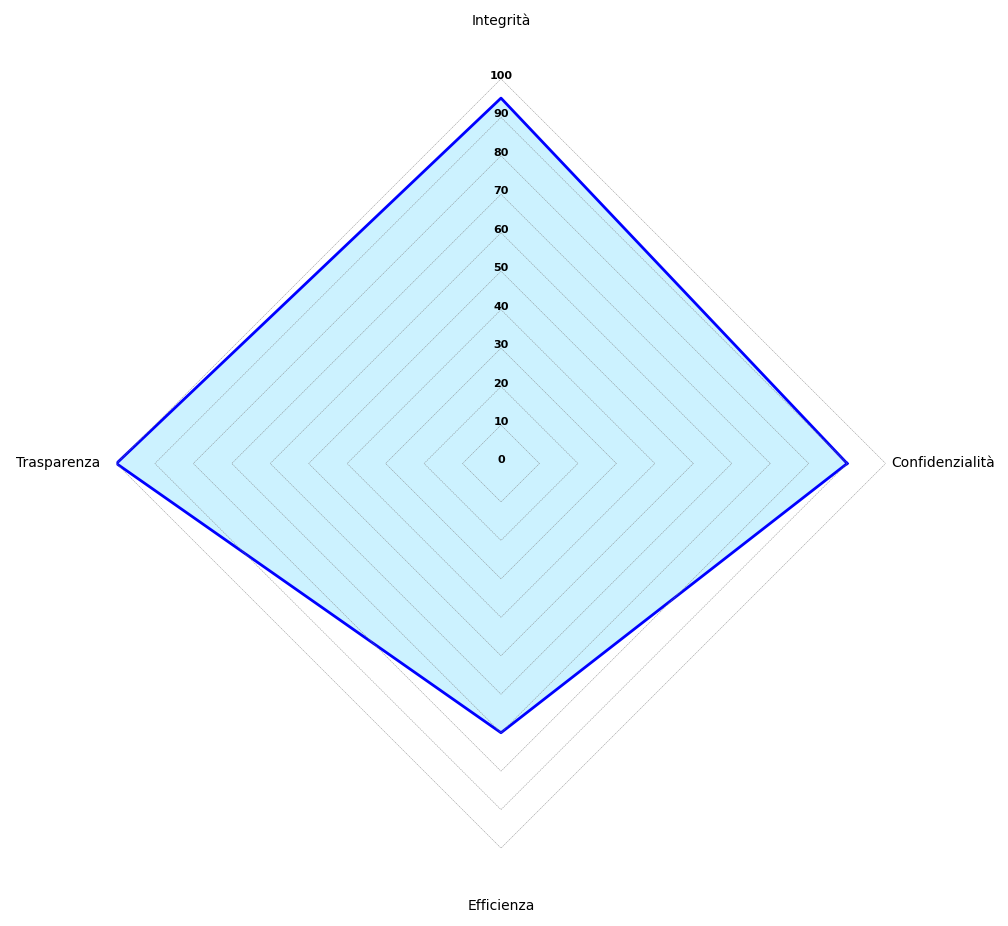
\includegraphics[width=1 \textwidth]{radar.png}
        \caption{Grafico radar relativo alle proprietà}
        \label{radar-graph-properties}
    \end{figure}